\section{Model fitting and likelihood analysis}\label{sec:fitting}

\begin{figure}
\centering
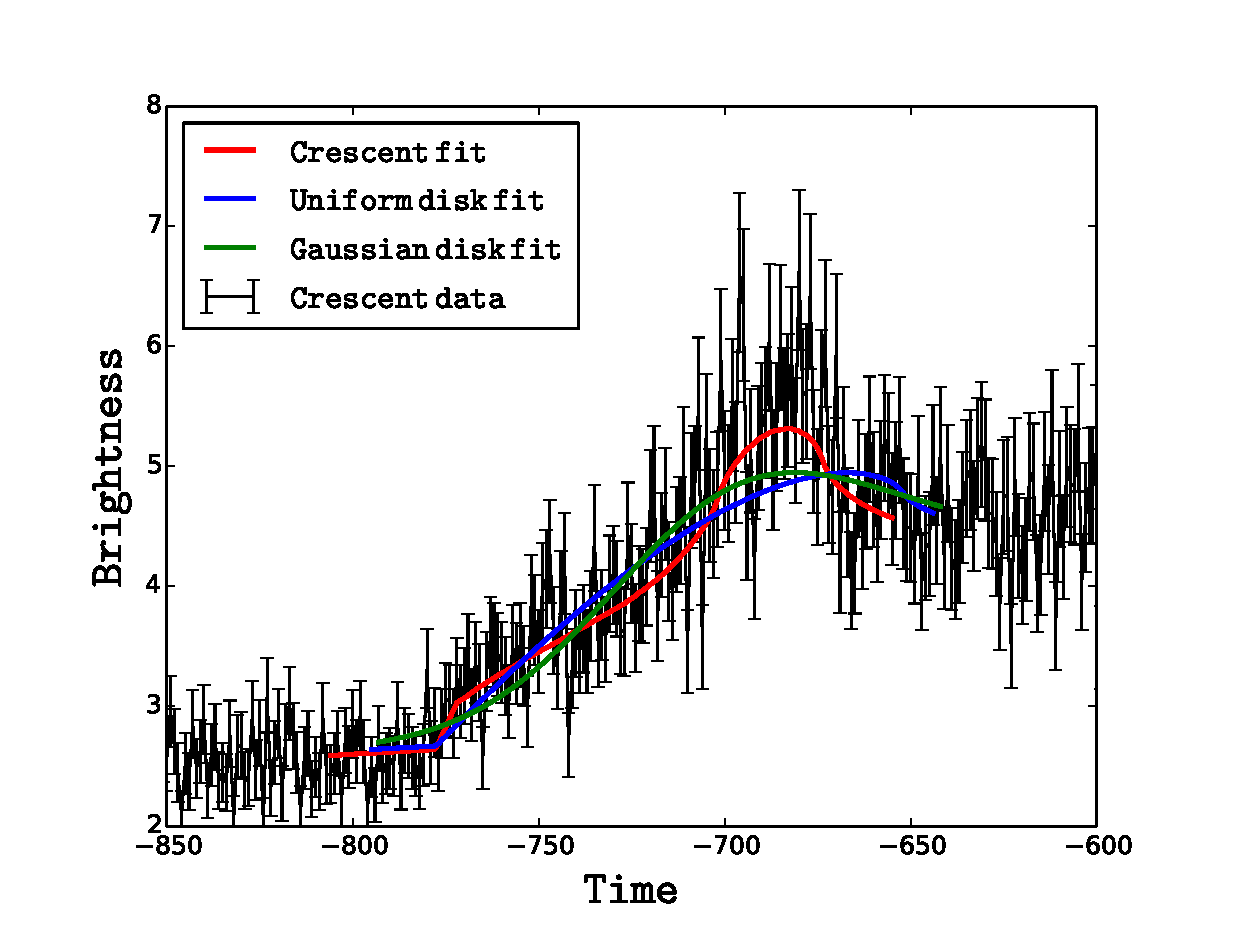
\includegraphics[width=0.9\hsize]{plots/data_cc.eps}
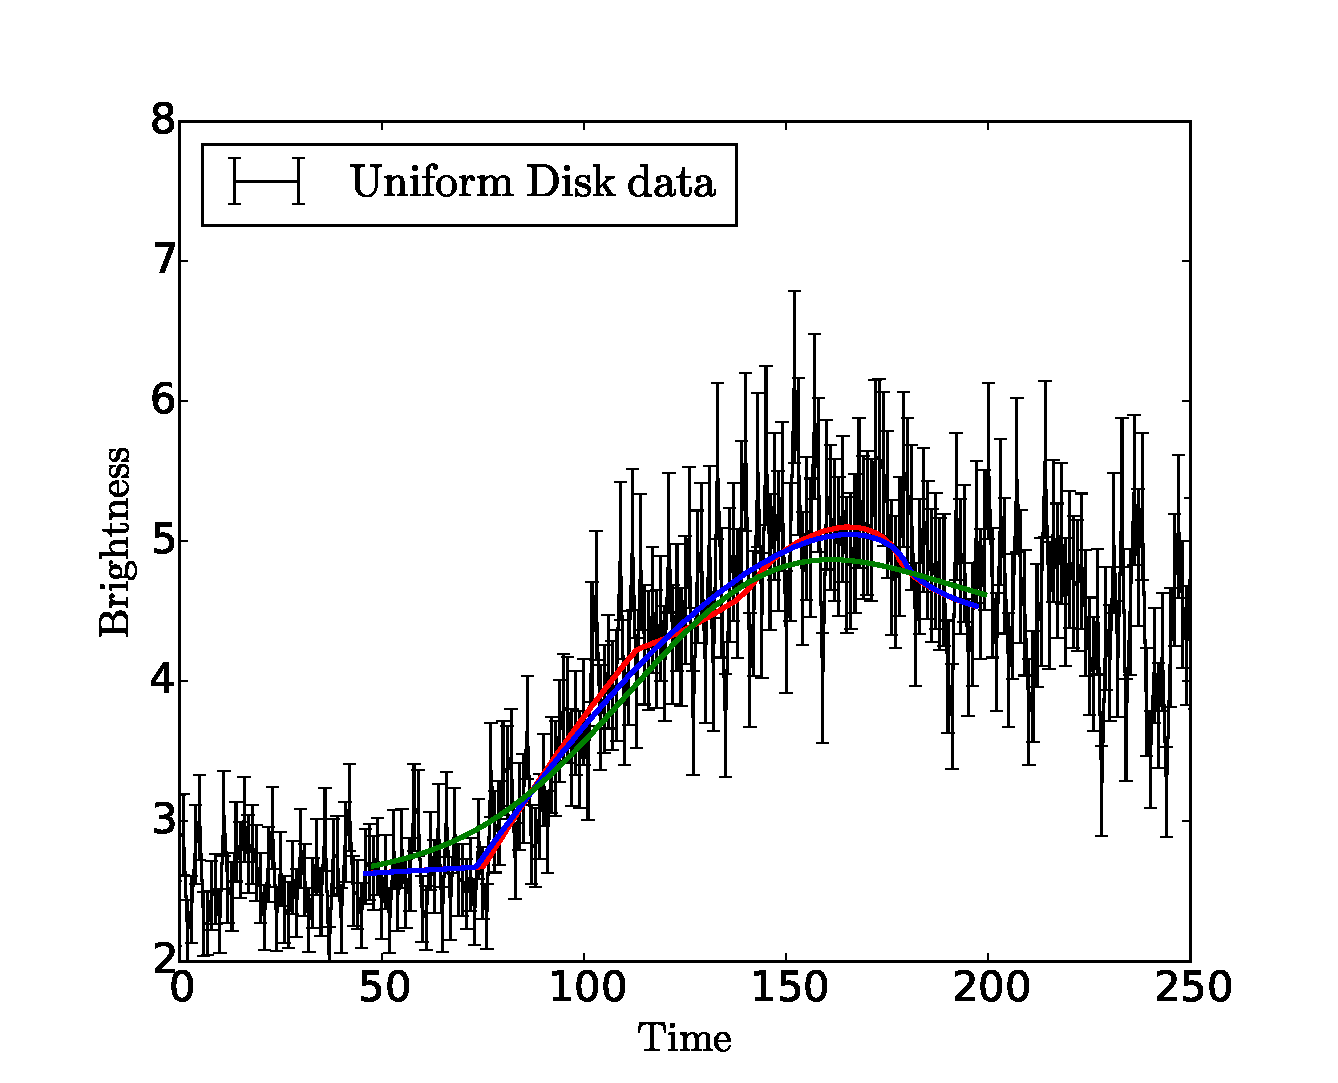
\includegraphics[width=0.9\hsize]{plots/data_dd.eps}
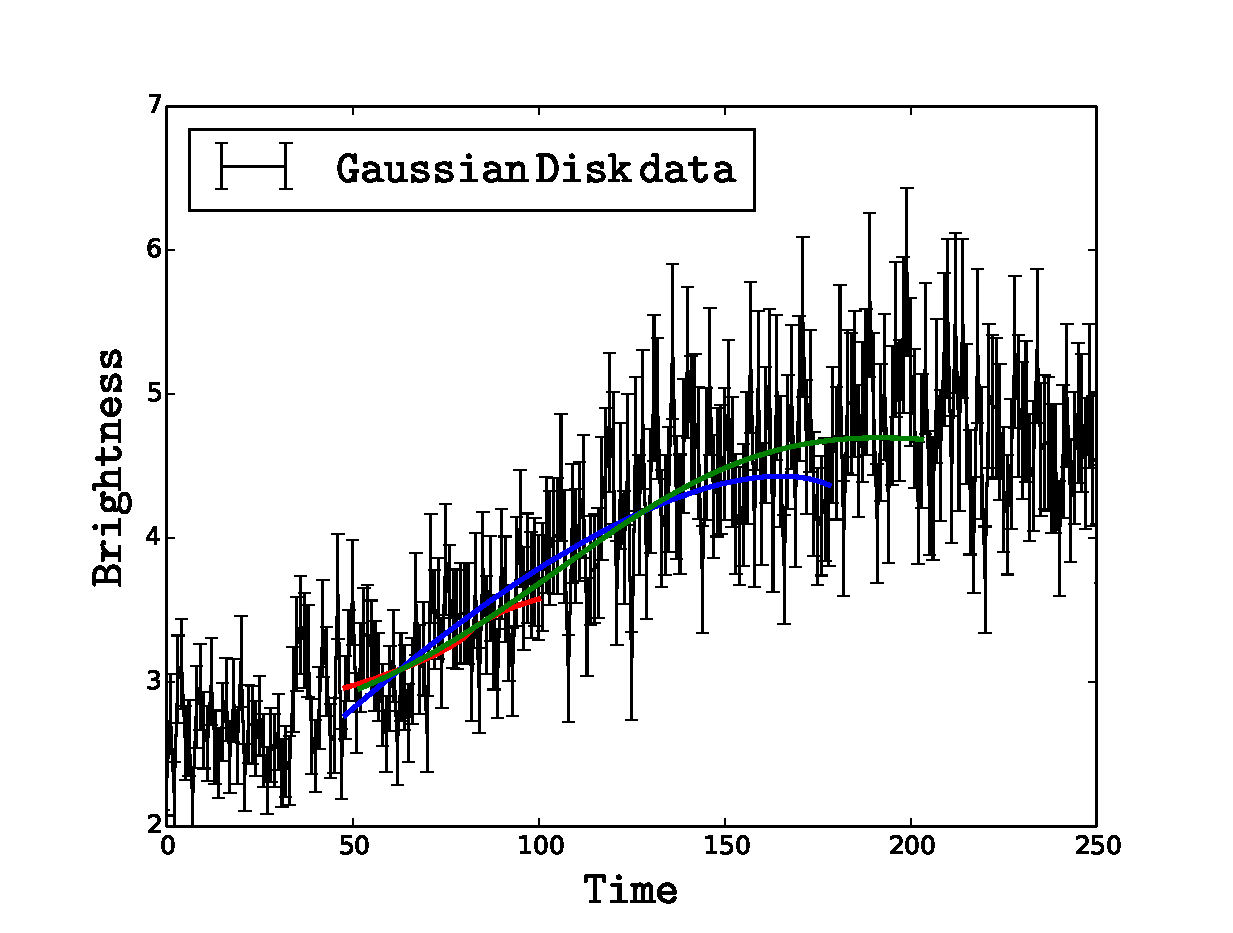
\includegraphics[width=0.9\hsize]{plots/data_gg.eps}
\caption{\label{fig:datafitting} Three different mock datasets with
  three different parameterisations fitted to each --- crescent (red),
  uniform-disk (blue) and Gaussian disk (green).}
\end{figure}


\begin{figure}
\centering
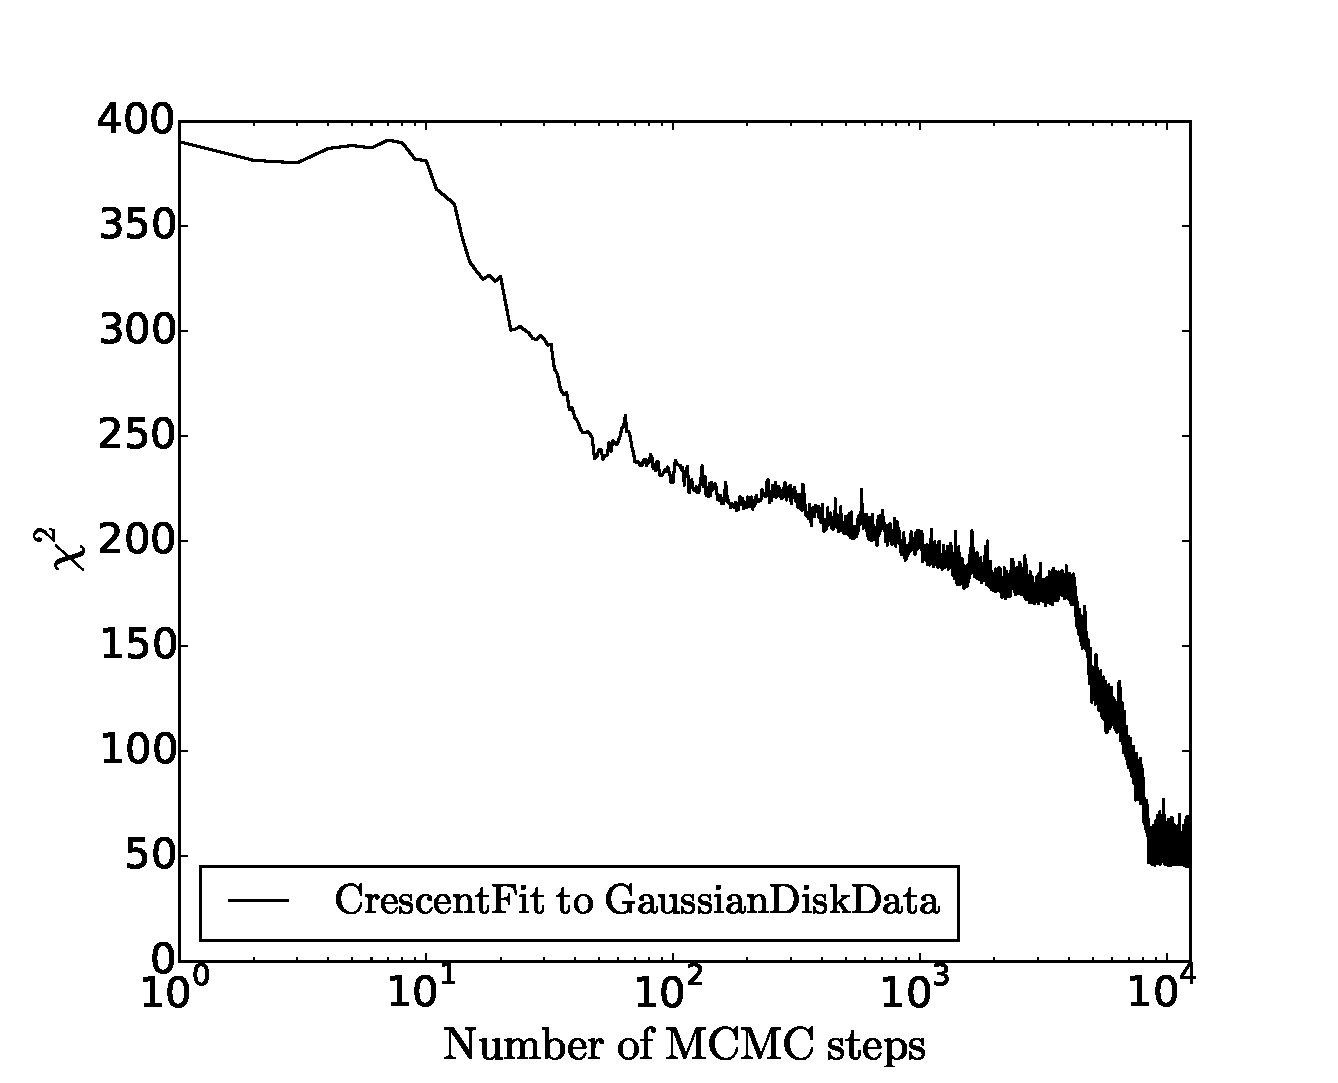
\includegraphics[width=0.9\hsize]{plots/burnin_cg.eps}
\caption{\label{fig:datafitting} The $\chi^2$ of each step of the full
  MCMC for one case.}
\end{figure}




\begin{figure}
\centering
  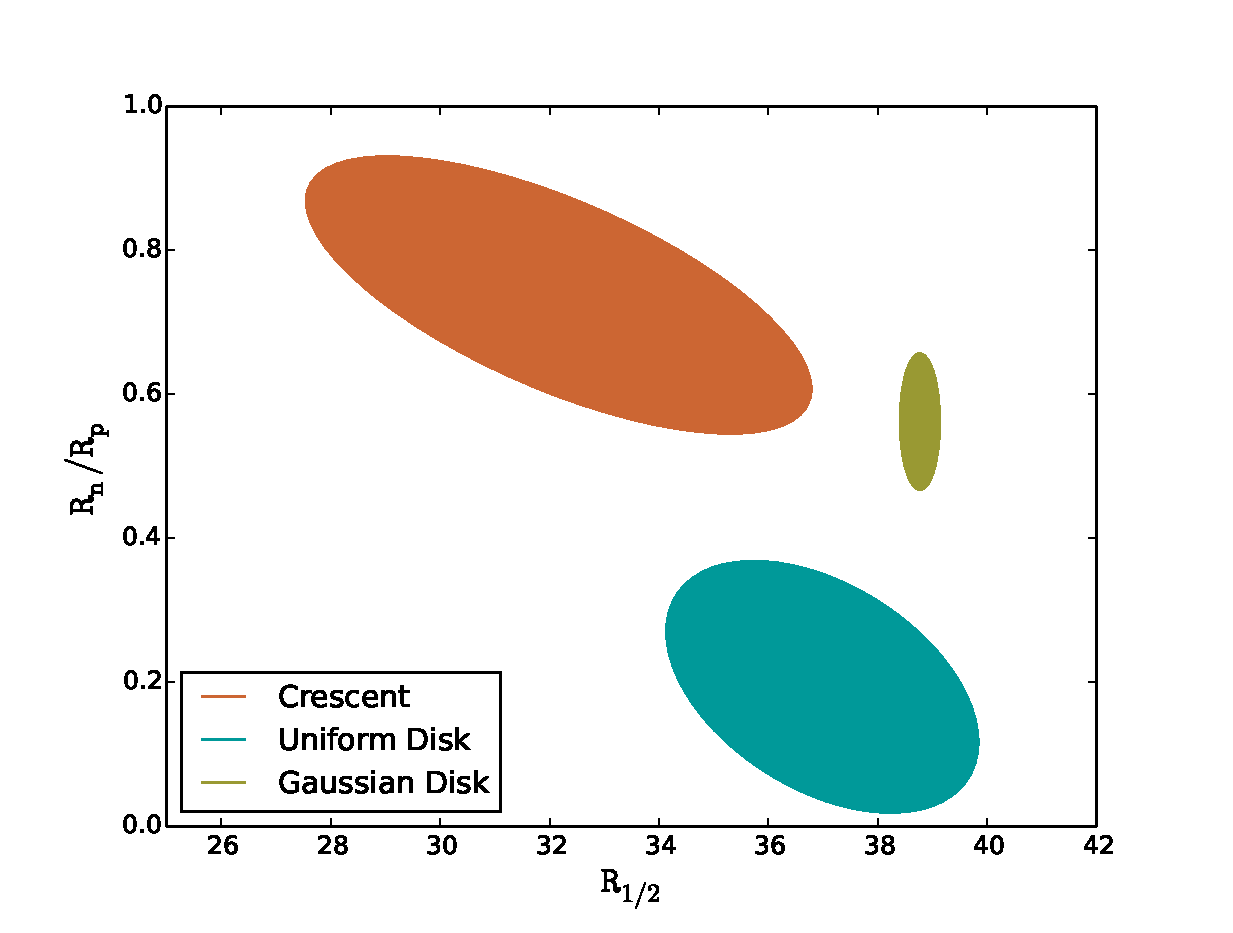
\includegraphics[width=0.9\hsize]{plots/Rhalf_RnRp.eps}
  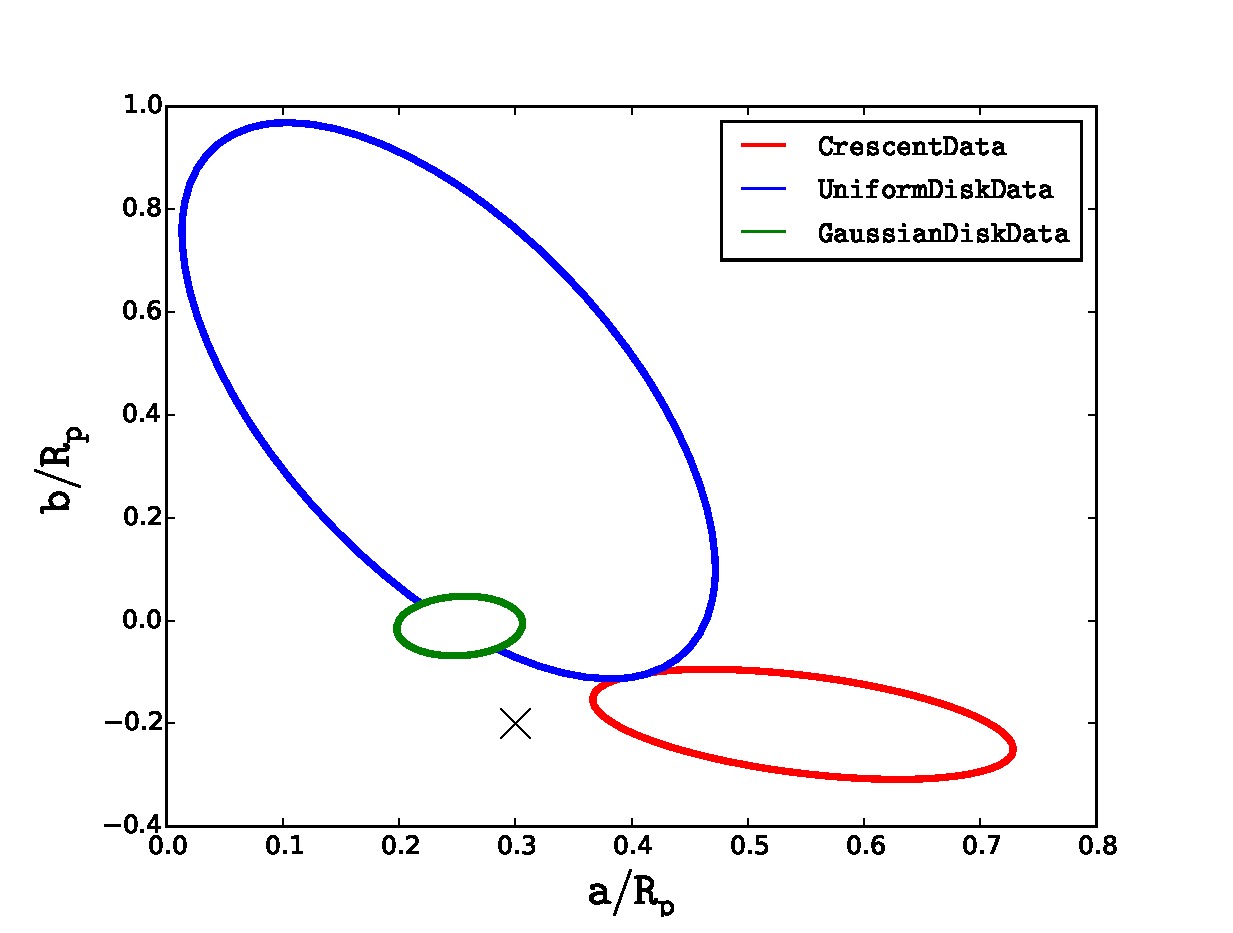
\includegraphics[width=0.9\hsize]{plots/aRp_bRp.eps}
\caption{\label{fig:mcmc} The 2$\sigma$ contours (or error ellipses)
  of the crescent model when fitting with the three different
  datasets.}
\end{figure}

\begin{figure}
\centering
  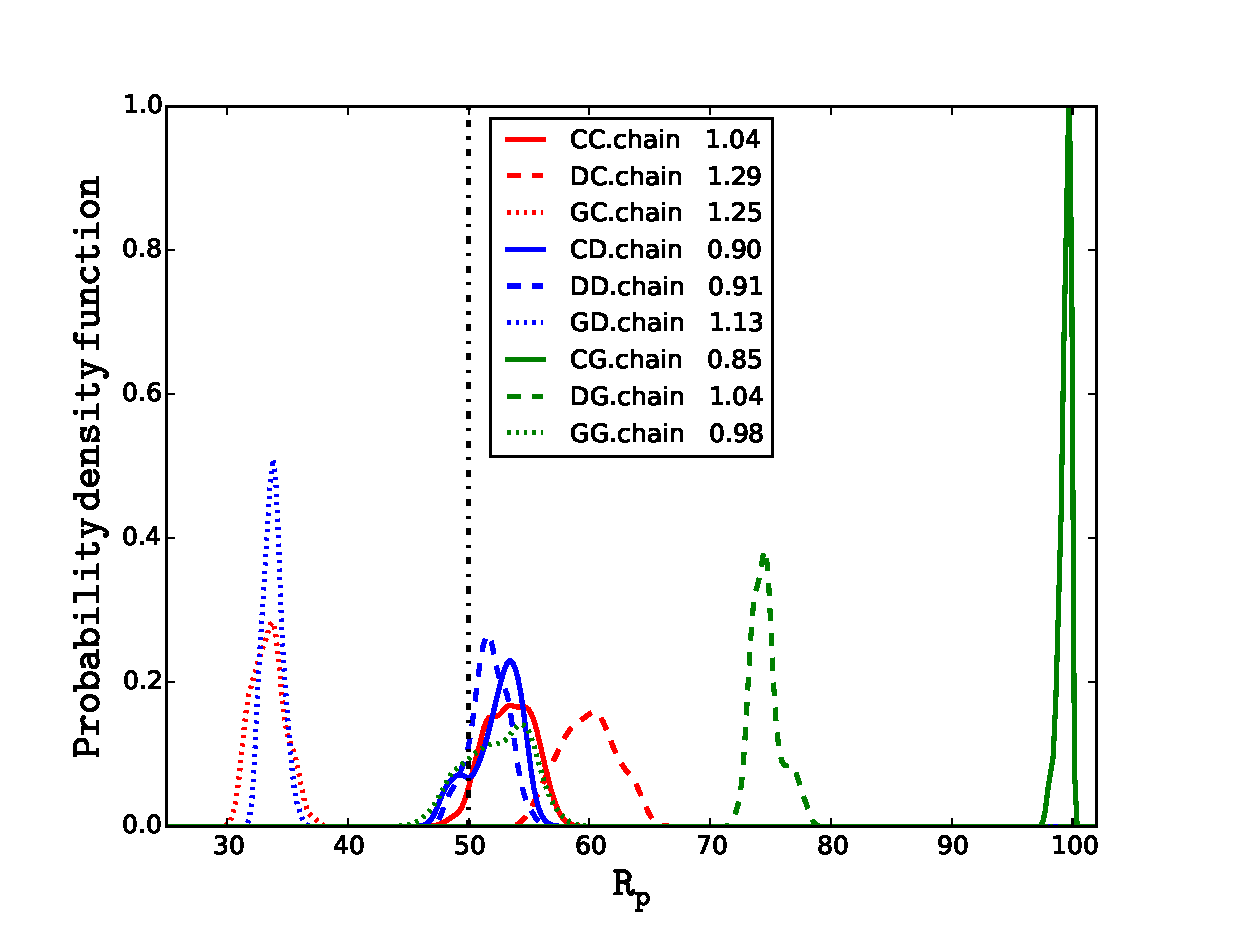
\includegraphics[width=0.9\hsize]{plots/Rp4all.eps}
\caption{\label{fig:mcmc} Posterior probability distribution for size
  of the source, $R_p$. Same color represeents the same dataset
  whereas same line style corresponds to same model fit. In the legend
  showing the reduced $\chi^2$ of the best fit in each case.}
\end{figure}


In this section, we attempt to mock three datasets, each for crescent, uniform-disk and Gaussian disk case for a given fiducial parameters and contaminate it with systematic and random noise, and fit \& recover the model parameters. Broadly we have 9 cases to discuss, we name these nine cases as different permutations (couplet) of three letters C, D and G for Crescent, Uniform-Disk and Gaussian Disk case respectively. The first letter of the couplet represents the fit model and the second represents the dataset. For example, CG represents the case where we fit Gaussian disk data to a crescent model. Similarly, DC respresents the case when crescent data is being fit with uniform-disk model. We explored the parameter space and carried out a likelihood analysis on all three parameter sets using Markov-chain Monte-Carlo (MCMC).

\subsection{Mock datasets and model parameters}
The datasets for each source model is in the form of light curves, the brightness of the source observed at different time. Figure \ref{fig:datafitting} shows the three datasets. These datasets are generated using the magnification map shown in figure \ref{fig:magnification_map} if the source of the respective model moves from point C to B. The data assumed was very  ideal, including 250 different data points at regular interval of time. We added Gaussian random noise to this dataset of width 10\% of the brightness at the respective time, which makes the signal to noise of about $\sim$150. After adding random noise, the three datasets are looking highly contaminated and no clear intuitive behaviour of fit can be seen. 

The fiducial model assumed to generate these mock datasets are:
\begin{equation}
	[R_p, R_n, a, b] = [50.0, 30.0, 15.0, 10.0]  \ \ \ \rm{for\ Crescent\ model},
	\label{eqn:cp}
\end{equation}
\\
where, $R_p$ and $R_n$ are the radius of outer and inner circles of the crescent respectively and $a$ and $b$ are the coordinates of the inner circle center with center of outer circle as the origin.

\begin{equation}
	R_p = 50.0 \ \ \ \rm{for\ Uniform\ disc\ model}
\end{equation}

\begin{equation}
	R_p = 50.0 \ \ \ \rm{for\ Gaussian\ disk\ model}
\end{equation}
\\
where, $R_p$ being the size of the uniform disc and Gaussian disc source model. We also have some nuisance parameters in all these cases: the beginning of the event (I), the end of the event (E), normalisation of the lightcurve (N). We marginalised over all these nuisance parameters. When we kept these three nuisance parameters free to vary in MCMC, it adapts to the amount of data for which the maximum likelihood is most optimal to find out. We talk more about this adaptaion in the next section. Secondly, We try to fit the these datasets for a crossing of the source from a different caustic, in this case, from point A to B in figure \ref{fig:magnification_map}. This adds a natural systematic in the dataset and the data is no more ideal. With these three characterstics -- random noise, systematic noise and nuisance parameters -- we make the dataset very general and highly contaminated to mock the real observations.

The aim of this exercise was to explore the degeneracies in  various model parameters and recover the correct fiducial model assumed from a highly contaminated dataset. Also, if it is possible that one can simply distinguish between circularly symmetric and asymmetric sources or uniform and Gaussian sources on the basis of maximum likelihoods. 

\subsection{Fitting with crescent model}

The main results of the MCMC are shown in figure \ref{fig:mcmc}. In the top row, we show the nine probability density function of recovered size of the source ($R_p$) and its half light radius ($R_{1/2}$) (left and right respectively). The legend of top-left panel has information about the datasets, fitting model and best fit also applicable to top-right panel for $R_{1/2}$. The name of the legend has the same convention as explained in the previous section. The number accompanying the name of the legend is the best fit reduced $\chi^2$. We follow the convention of red, blue and green color for crescent, uniform disc and Gaussian disk datasets respectively whereas the fitting model is represented by different kind of curves: solid, dashed and dot-dashed respectively.



First we explored the parameter space for crescent source model and run its likelihood exploration for three different datasets. Here we have four interesting parameters as given by equation \ref{eqn:cp} and we marginalise over all other nuisance parameters. Three solid curves in top row of figure \ref{fig:mcmc} represents the resulting likelihood of $R_p$, the overall size of the crescent source fitted with three different datasets. We also show results for half light radius $R_{1/2}$.

\begin{enumerate}

\item Crescent data: This is the true case for crescent model fitting. The red solid line represents this case in upper panels of figure \ref{fig:mcmc} as 1D probability density function marginalised over all other parameters. The true value of $R_p$ can be recovered within 2$\sigma$ level with an accuracy up to 10\%. Also the best fit to the data is shown in red line in upper-left panel of figure \ref{fig:datafitting}. It is a very good fit which also represents a reduced $\chi^2$ close to unity (1.04). The orange contour in the lower panels of figure \ref{fig:mcmc} showing the 2D marginalised error ellipses. There is a certain degeneracy in $R_{1/2}$ and $R_n/R_p$ parameters but all the values are well recovered. 

\item Uniform disk data: In this case, we tried to fit crescent model to disk data. The solid blue line in top row panels and cyan contours in bottom row panel represent this case. The best fit reduced $\chi^2$ (0.90) is better than the previous case as the data is generated by one parameter only and fitting with four parameter that can also model the noise. This can also be seen in the best fit to the data, figure \ref{fig:datafitting} red line in top-right panel, where the curve seems to fit the noise as well. The maximum likelihood (and also average likelihood) is achieved close to $R_n = 0$, as already mentioned, this is intuitive as well. The other paramters, $a$ and $b$ are quite arbitary and highly uncertain. 

\item Gaussian disk data: In this case, Gaussian disc data is fited with crescent model. The solid green line in top row panels and green contours in bottom row panels of figure \ref{fig:mcmc} represent this case. By looking at figure \ref{fig:mcmc}, it can be seen that all the parameters can be constrained really well, even the best fit $\chi^2$ is much better than other two cases (0.85) which also shows a bit of over-fitting problem. However, this is misleading. The reason for these strong constraints is that the full data is not at all fitted, in this case the nuisance parameters are rejecting most of the data during the progress of MCMC. This can be seen in figure \ref{fig:datafitting} bottom-left panel in red line, where the best fit model is fitted only in very small range of data, even before the actual incidence happened. In other words, MCMC is unable to converge in this case and the only way to achieve better likelihood is to reject data points. This can be seen in bottom-left panel of figure \ref{fig:datafitting}. The $\chi^2$ keep on reducing through the span of MCMC chain and not saturating anywhere. 

\end{enumerate}

Therefore we can conclude that by fitting with crescent source model, one can recover the parameters very well if the dataset is generated by crescent source model. The uniform disk source model can also be recovered very well for the overall shape of the disk, as the latter is the special case of the former, but other parameters like $a$ and $b$ are arbitary and $R_n \sim 0$. No convergence can be achieved for data generated by Gaussian disk model. 

Please notice that in top row of figure \ref{fig:mcmc}, the height of the peaks does not represents the likelihood, it is just ensuring that the area under the curve is unity. The likelihood can be estimated from the number in the legend which is the best fit $\chi^2$.


 In the bottom rows we show three contours, for three different datasets (same color convention) fitted with crescent parameters only because this is the only case with more than one relevant parameter. Note that we plotted the 2D ellipses with principal component analysis of the MCMC and this is the reason they are perfect ellipses and not arbitary shape.

\subsection{Fitting with uniform disc model}
In this case, we have only one interesting parameter to fit, the outer radius of the uniform disc with uniform intensity. When fitting with the true case, the uniform disk data itself (dashed blue line in upper panels of figure \ref{fig:mcmc}), the best fit $\chi^2$ is very good (0.91) and also it recovers the true value of $R_p=50$. When fitting with crescent data (dashed red line), the maximum likelihood shifts towards higher values of $R_p$ as compared to the fiducial value. This is justified and intuitive as $R_n \sim > 0$. Also the best fit reduced $\chi^2$ is 1.29 which is much worse than the true case. However, when fitting with Gaussian disc data (dashed green line), the best fit reduced $\chi^2$ is still very low but still worse than the true case. However, it can be seen in figure \ref{fig:datafitting} (blue line bottom-left panel) that in this case also many points are rejected in order to gain better likelihood.

Therefore we conclude here that looking at the maximum likelihood one can identify the true dataset and also recover the true values of the parameters. 


\subsection{Fitting with Gaussian disc model}
In the last case, we fit Gaussian disc model to the three datasets (dot-dashed curves in top panels of figure \ref{fig:mcmc}). In this case, when fitted with the true case, Gaussian disc dataset, the true parameters can be recovered at the correct value and also the best fit reduced $\chi^2$ is close to unity (0.98). In all other cases the maximum likelihood is much worse and also the recovered values of $R_p$ are many $\sigma$ away.

Hence, in this case also by looking at the maximum likelihood true case can be identified and parameters can be restored correctly.



\subsection{Conclusions and interpretations}
The main results of this work is given in figure \ref{fig:mcmc} and described in the previous section. Here we try to interpret those results and conclude the take away message.

Lets assume that an ideal telescope observes a quasar for a long time and we get the lightcurve  and one can clearly see the event of caustic crossing in the light curve. Now one wants to extract the true shape of the source. To comment more specifically, lets assume three cases when the true shape of the source is: crescent, uniform disc or Gaussian disc:

\begin{enumerate}

\item Crescent shape source: if one tries to fit this curve with crescent model, the maximum likelihood will be good and one can recover the true parameters with good precision. In the other two cases, the maximum likelihood will be bad. Hence this shape can be recovered very well by trusting the maximum likelihood analysis.
\item Uniform disc shape source: if one tries to fit this curve with Gaussian disk model, the likelihood will be very little to disprove it, however, the other two models are inditinguishable with nearly the same likelihood. At this point it does not matter as one can obtain the true result from both uniform disk and crescent model.
\item Gaussian disc shape source: if one tries to fit this curve with uniform disk model or crescent model, again likelihood will discard this choice. Again the maximum likelihood analysis will point towards the best fitted true model.
\end{enumerate}

Therefor, we conclude that maximum likelihood analysis can be well trusted in order to recover true shape and recovering the corresponding parameters. This will provide the accurate recovery of the model parameters, however, for more precise recovery, one rely on precise measurements of the lightcurve. 

 
